\section{Results}

\subsection{Determining the appropriate $\Gamma$}

In this section, we optimize the aircraft configuration for a given payload and range with no uncertainty, box uncertainty and ellipsoidal uncertainty, and attempt to determine the value of $\Gamma$ that gives the best trade-off between robustness and optimality for the RO formulations. The problems have been solved with box uncertainty and ellipsoidal uncertainty for a range of $\Gamma$. For each of the robust solutions, both the estimated probability of failure and the objective cost have been plotted in Figures~\ref{fig:probOfFail_vs_Gamma} and \ref{fig:W_f_vs_Gamma} respectively.

\begin{figure}[h]
\centering
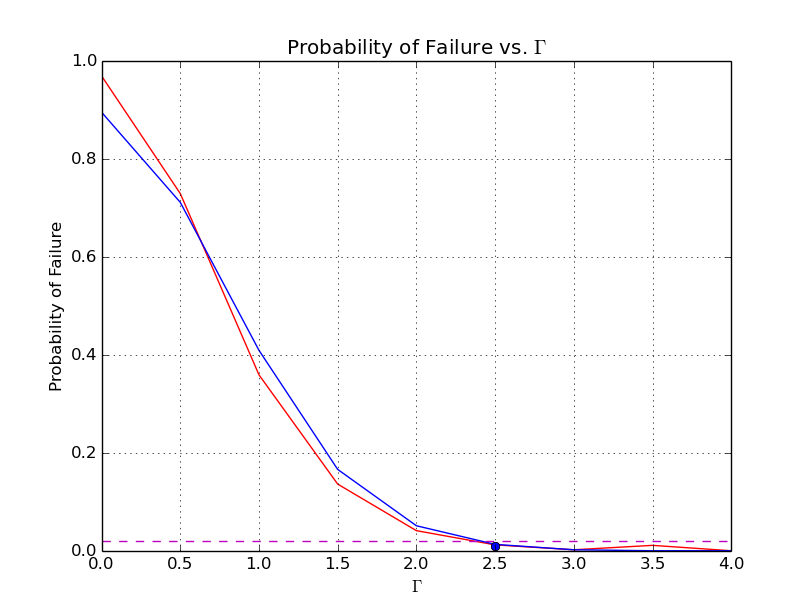
\includegraphics[width=0.6\textwidth]{probOfFail_vs_Gamma.png}
\caption{The probability of failure vs. $\Gamma$. Note the high ($\geq$ 90\%) probability of failure for the non-robust ($\Gamma$ = 0) solutions. The difference in the probability of failure for the non-robust cases is due to subtle numerical errors in the evaluation of the solution obtained for the ellipsoidal uncertainty set.}
\label{fig:probOfFail_vs_Gamma}
\end{figure}

\begin{figure}
\centering
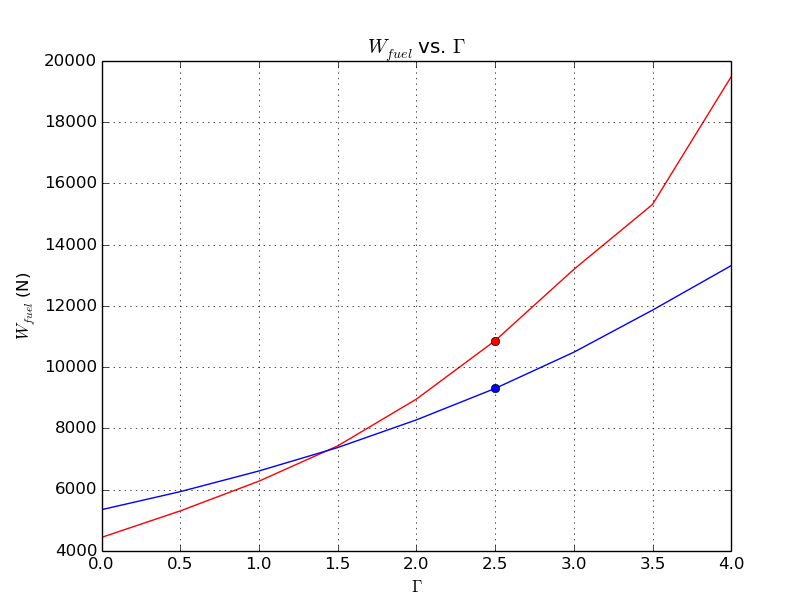
\includegraphics[width=0.6\textwidth]{W_f_vs_Gamma.png}
\caption{Fuel weight vs. $\Gamma$ demonstrates the deterioration of the objective as we protect against larger variation of parameters.}
\label{fig:W_f_vs_Gamma}
\end{figure}

We define the probability of failure to be the probability of constraint violation in 1000 samples of the uncertain parameters from a normal distribution with the specified $3\sigma$ uncertainties. For this problem, we allow for less than 2\% probability of failure, shown by the magenta line in Figure~\ref{fig:probOfFail_vs_Gamma}, and consider half-integer values of $\Gamma$. This corresponds to a $\Gamma$ of 2.5 for both the box uncertainty and the ellipsoidal uncertainty, resulting in 1.2\% and 1.3\% probability of failure respectively.

We know that elliptical uncertainty sets are less conservative than box uncertainty sets, especially when we have a large number of uncertain parameters per constraint. The results we got are somehow expected, and this would show how designing using uncertainty sets is better than using margins which are - in the best case - somehow similar to box uncertainty sets.

\subsection{Optimization results}

At the chosen values of $\Gamma$, the results of the optimization are shown in Table~\ref{tab:results}.

\begin{table}[!h]
\begin{center}
\caption{\label{tab:results} SP Aircraft Optimization Results }
\begin{tabular}{c c c c}
\hline
Free variable & No Uncert. & Box [$\Gamma = 2.5$] & Ellipsoidal [$\Gamma = 2.5$] \\
\hline
$L/D$ & 23.8 & 16.41 & 17.3 \\
$AR$ & 12.0 & 5.016 & 6.56 \\
$Re$ & 4.76e6 & 1.16e7 & 9.55e6 \\
$S (m^2) $ & 21.6 & 72.21 & 58.9 \\
$V (m/s)$ & 51.0 & 47.73 & 48.6 \\
$T_{flight} (hr)$ & 17.46 & 18.1 & 17.2 \\
$W_w$ & 2440 & 6278 & 5470 \\
$W_{w_{strc}} (N)$ & 1210 & 1570 & 1650 \\
$W_{w_{surf}} (N)$ & 1230 & 1592 & 3820 \\
$V_{f_{avail}} (m^3)$ & 0.566 & 1.794 & 1.48 \\
$V_{f_{fuse}} (m^3)$ & 0.461 & 0.891 & 0.903 \\
$V_{f_{wing}} (m^3)$ & 0.105 & 0.9027 & 0.582 \\
$CDA_0 (m^2)$ & 0.0461 & 0.0891 & 0.0903 \\
\hline
E[Objective] & No Uncert. & Box [$\Gamma = 2.5$] & Ellipsoidal [$\Gamma = 2.5$] \\
\hline
$W_{fuel} $ (N) & 4430 & 10858 & 9299 \\
\hline
P[failure] & No Uncert. & Box [$\Gamma = 2.0$] & Ellipsoidal [$\Gamma = 2.5$] \\
\hline
\% & 92 & 1.2 & 1.3\\
\hline
\end{tabular}
\end{center}
\end{table}

\subsection{Comparing results for different objective functions}

\begin{figure}
\caption{Design optimization of the aircraft with no uncertainty for 3 different objective functions. The red, blue and yellow correspond to $\frac{W_f}{L/D}$, $D$, $W_f$ and objectives respectively.}
\begin{center}
\begin{tikzpicture}[scale=0.75]
\tkzKiviatDiagram{$\frac{W_f}{L/D}$,$D$,$W_f$}
%solve for {W_f}{L/D}
\tkzKiviatLine[thick,
color=red,
mark=ball,
ball color=red,
mark size=3pt,opacity=.2,
fill=red!20](154.4/25,414.2/75,5180/700)
%solve for D
\tkzKiviatLine[thick,
color=blue,
mark=ball,
mark size=3pt,
fill=blue!20,
opacity=.5](161.8/25,400/75,5129/700)
% solve for {W_f}
\tkzKiviatLine[thick,
color=yellow,
mark=ball,
mark size=3pt,
fill= yellow!20,
opacity=.5](190.2/25,463.4/75,4536/700)
\label{fig:spiderplotnoUncert}
\end{tikzpicture}
\end{center}
% tkz-kiviat documentation here in FRENCH: http://mirror.jmu.edu/pub/CTAN/macros/latex/contrib/tkz/tkz-kiviat/doc/TKZdoc-kiviat-main.pdf
\end{figure}

To further demonstrate the capabilities of robust SPs in aircraft design, we performed the optimization of the aircraft with no uncertainty and ellipsoidal uncertainty ($\Gamma = 2.5$) for two more objective functions, and plotted the results on spider plots. Spider plots are useful because they allow engineers to find non-dominated solutions among the solutions that lie on the Pareto frontier of potential objective functions. The objective functions chosen for this analysis were fuel burn over lift-to-drag ratio ($\frac{W_f}{L/D}$), drag ($D$), and fuel burn ($W_f$).

In the spider plots in Figures \ref{fig:spiderplotnoUncert} and \ref{fig:spiderplotEllUncert}, none of the solutions are non-dominated for both the no uncertainty and ellipsoidal uncertainty cases. In a GP, it is not possible that one of the solutions is non-dominated since the solutions are globally optimal. But since there is no guarantee in optimality for SPs, it is possible to find non-dominated solutions if the obtained solution is a local optimum.

In the case where there is no non-dominated solution such as this one, we take the internal areas of the triangle formed by each optimization to be the figure of merit. The smaller the area in the triangle, the higher the performance of the proposed solution. In the no uncertainty case shown in Figure~\ref{fig:spiderplotnoUncert}, the red solution with the objective of $\frac{W_f}{L/D}$ has the smallest internal area. In the ellipsoidal case shown in Figure~\ref{fig:spiderplotEllUncert}, the blue solution with the objective of $D$ has the smallest internal area.

This is an interesting result, because the presence of an uncertainty set is shown to affect the efficacy of different objective functions to obtain solutions with the best overall performance. The differences between the objective functions in the simple aircraft design problem are minute, because the different potential objectives have a high degree of coupling. It is likely that, if the three objective functions didn't have high degree of coupling, that the internal areas of the solution triangles may differ more significantly.

\begin{figure}[H]
\caption{Design optimization of the aircraft with ellipsoidal uncertainty ($\Gamma = 2.5$) for 3 different objective functions. The red, blue and yellow correspond to $\frac{W_f}{L/D}$, $D$, $W_f$ and objectives respectively.}
\begin{center}
\begin{tikzpicture}[scale=0.75]
\tkzKiviatDiagram{$\frac{W_f}{L/D}$,$D$,$W_f$}
%solve for {W_f}{L/D}
\tkzKiviatLine[thick,
color=red,
mark=ball,
ball color=red,
mark size=3pt,opacity=.2,
fill=red!20](568.6/100,1051/150,13500/1500)
%solve for D
\tkzKiviatLine[thick,
color=blue,
mark=ball,
mark size=3pt,
fill=blue!20,
opacity=.5](587/100,1024/150,13100/1500)
% solve for {W_f}
\tkzKiviatLine[thick,
color=yellow,
mark=ball,
mark size=3pt,
fill= yellow!20,
opacity=.5](687.9/100,1155/150,11900/1500)
\label{fig:spiderplotEllUncert}
\end{tikzpicture}
\end{center}
% tkz-kiviat documentation here in FRENCH: http://mirror.jmu.edu/pub/CTAN/macros/latex/contrib/tkz/tkz-kiviat/doc/TKZdoc-kiviat-main.pdf
\end{figure}